\documentclass[border=6pt]{standalone}
\usepackage{amssymb}
\usepackage{amsmath}
\usepackage{tikz}
\usetikzlibrary{positioning, decorations.pathreplacing, calc}

\definecolor{cnavy}{HTML}{0E2747}
\definecolor{corange}{HTML}{E8573F}
\definecolor{cgreen}{HTML}{3B9B6D}
\definecolor{cslate}{HTML}{5B6680}
\definecolor{cmuted}{HTML}{9B9484}
\definecolor{ccream}{HTML}{FAFAF6}

\begin{document}
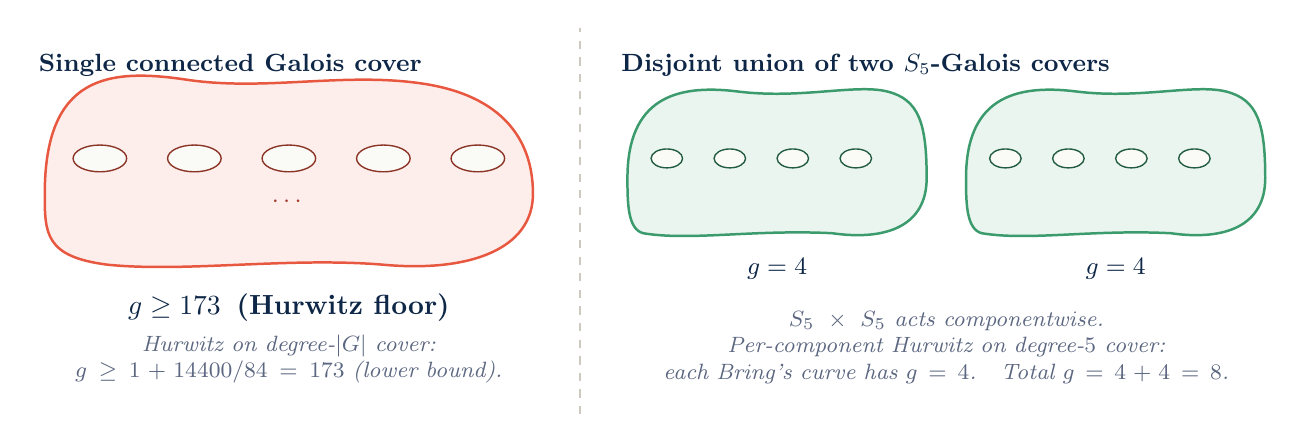
\begin{tikzpicture}[
  font=\sffamily,
  surface/.style={
    draw=#1, fill=#1!10, line width=0.9pt
  },
  hole/.style={
    draw=#1!60!black, fill=ccream, line width=0.5pt
  }
]

% ============================================================
% LEFT panel: single high-genus cover
% ============================================================
\node[anchor=north west, cnavy, font=\bfseries\small]
  at (0, 4.4) {Single connected Galois cover};

% Outer blob with 5 visible handles (stylised g = 173)
\draw[surface=corange]
  (0.2, 2.5) .. controls (0.2, 4.0) and (1.0, 4.1) ..
  (2.0, 3.95) .. controls (3.0, 3.8) and (4.0, 4.05) ..
  (5.0, 3.9) .. controls (6.0, 3.75) and (6.4, 3.2) ..
  (6.4, 2.5) .. controls (6.4, 1.8) and (5.6, 1.5) ..
  (4.5, 1.6) .. controls (3.3, 1.7) and (2.0, 1.5) ..
  (1.0, 1.6) .. controls (0.2, 1.7) and (0.2, 2.0) ..
  cycle;

% Five handle ellipses
\foreach \x in {0.9, 2.1, 3.3, 4.5, 5.7} {
  \draw[hole=corange] (\x, 2.95) ellipse (0.34cm and 0.17cm);
}

% "..." between handles to suggest many more
\node[corange!70!black, font=\bfseries\small, anchor=center]
  at (3.3, 2.4) {$\cdots$};

\node[cnavy, font=\bfseries\normalsize, anchor=center]
  at (3.3, 1.05) {$g \geq 173$\enspace (Hurwitz floor)};

\node[cslate, font=\itshape\footnotesize, anchor=center, align=center, text width=6.4cm]
  at (3.3, 0.4) {Hurwitz on degree-$|G|$ cover:\\
  $g \geq 1 + 14400 / 84 = 173$ (lower bound).};

% Divider between panels
\draw[cmuted!50, line width=0.6pt, dashed]
  (7.0, -0.3) -- (7.0, 4.6);

% ============================================================
% RIGHT panel: two-component split
% ============================================================
\node[anchor=north west, cnavy, font=\bfseries\small]
  at (7.4, 4.4) {Disjoint union of two $S_5$-Galois covers};

% First component blob (left)
\draw[surface=cgreen]
  (7.6, 2.7) .. controls (7.6, 3.7) and (8.2, 3.9) ..
  (9.0, 3.8) .. controls (9.8, 3.7) and (10.5, 3.9) ..
  (10.9, 3.8) .. controls (11.3, 3.7) and (11.4, 3.4) ..
  (11.4, 2.7) .. controls (11.4, 2.1) and (10.9, 1.9) ..
  (10.2, 2.0) .. controls (9.2, 2.05) and (8.4, 1.9) ..
  (7.8, 2.0) .. controls (7.6, 2.05) and (7.6, 2.4) ..
  cycle;
% 4 handles
\foreach \x in {8.1, 8.9, 9.7, 10.5} {
  \draw[hole=cgreen] (\x, 2.95) ellipse (0.20cm and 0.12cm);
}
\node[cnavy, font=\bfseries\small, anchor=center]
  at (9.5, 1.55) {$g = 4$};

% Second component blob (right) - identical shape, shifted
\draw[surface=cgreen]
  (11.9, 2.7) .. controls (11.9, 3.7) and (12.5, 3.9) ..
  (13.3, 3.8) .. controls (14.1, 3.7) and (14.8, 3.9) ..
  (15.2, 3.8) .. controls (15.6, 3.7) and (15.7, 3.4) ..
  (15.7, 2.7) .. controls (15.7, 2.1) and (15.2, 1.9) ..
  (14.5, 2.0) .. controls (13.5, 2.05) and (12.7, 1.9) ..
  (12.1, 2.0) .. controls (11.9, 2.05) and (11.9, 2.4) ..
  cycle;
\foreach \x in {12.4, 13.2, 14.0, 14.8} {
  \draw[hole=cgreen] (\x, 2.95) ellipse (0.20cm and 0.12cm);
}
\node[cnavy, font=\bfseries\small, anchor=center]
  at (13.8, 1.55) {$g = 4$};

\node[cslate, font=\itshape\footnotesize, anchor=center, align=center, text width=8.0cm]
  at (11.65, 0.55) {$S_5 \times S_5$ acts componentwise.\\
  Per-component Hurwitz on degree-$5$ cover:\\
  each Bring's curve has $g = 4$.\quad Total $g = 4 + 4 = 8$.};

\end{tikzpicture}
\end{document}
